% Chapter Template

% Main chapter title
%\chapter[toc version]{doc version}
\chapter{Background}

% Short version of the title for the header
%\chaptermark{version for header}

% Chapter Label
% For referencing this chapter elsewhere, use \ref{ChapterTemplate}
\label{Section2}

% Write text in here
% Use \subsection and \subsubsection to organize text
In this chapter, the relevant background needed for the work done in this thesis is presented, with an emphasis on 
the transformers architecture and tokenizers as well as the different models used to create them.
The principal goal of this chapter is to provide a background for the reader to understand the work done in this thesis, given that
the reader already has some basic understanding of the field at study, machine learning, neural networks and deep learning to name a few.


\section{Transformers}\label{Section2.1}
Introduced in the 2017 paper, ~\citet{AttentionIsAllYouNeed},
the transformers architecture have revolutionized the field of Natural Language Processing (NLP).
Transformers are encoder-decoder architectures that use a self-attention mechanism to learn the dependencies between the words in a sentence.
\begin{figure}
    \centering
      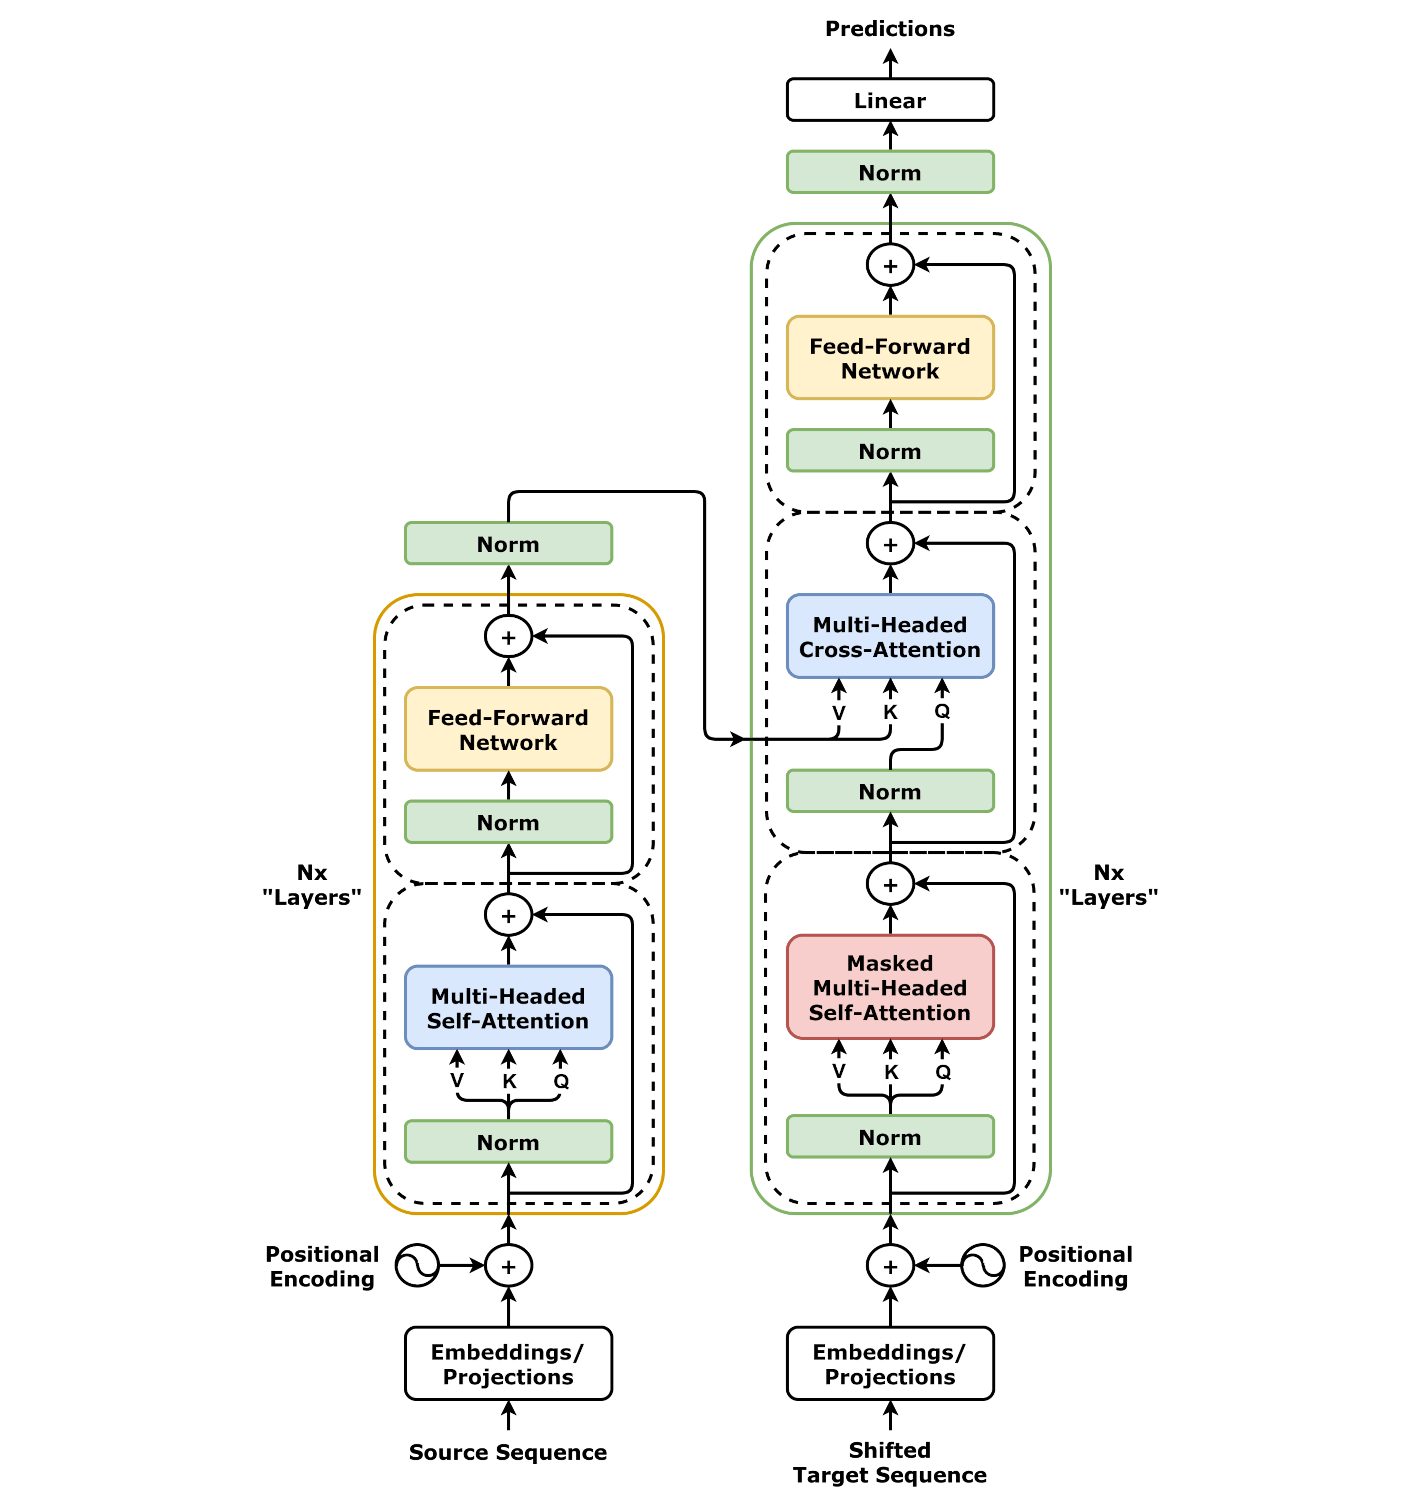
\includegraphics[width=0.5\columnwidth]{Transformers/full_architecture.png}
      \captionof{figure}{\label{fig:Transformers-FullArchitecture}Transformers Architecture}
\end{figure}


\subsection{Encoding}\label{Section2.1.1}
As seen in Figure~\ref{fig:Transformers-FullArchitecture}, the transformers architecture starts with encoding an input 
sequence into a sequence of vectors of fixed size. Each sequence is first split into tokens, which have been pre-trained on a large corpus of text to produce
the vectors of the encoding layer.

\subsection{Decoding}\label{Section2.1.2}
After obtaining the encoding of the input sequence, the decoder uses the self attention layer to learn the dependencies between the input tokens which 
updates the weights of the input tokens. This usually happens multiple times, in the hidden layers, and is later passed through a feed-forward layer.

After obtaining the final output of the Feed-forward layer, the decoder outputs a probability distribution over the vocabulary, made up of the initial tokens given as inputs.

\subsection{Attention Layer}\label{Section2.1.3}
As mentioned above, during the attention layer the model learns the dependencies between the input tokens. 
This is done by computing the attention weights for each token in the input sequence, which are then used to update the weights of the input tokens.
The attention weights are computed by multiplying the input tokens by a weight matrix, which is then passed through a softmax function to obtain the attention weights.

\section{Tokenizers}\label{Section2.2}
For a sequence of words to be processed by a transformer model, it must first be converted into something a computer can understand.
This is done by tokenizing the input sequence into a sequence of tokens.
On its most basic form, a tokenizer is a function that takes a sequence of words and returns a sequence of tokens.
These tokens can be obtained by different methods, such as splitting the sequence into words, splitting the sequence into characters, or using a pre-trained model to tokenize the sequence.

We will address some of the most common algorithm used to obtain the vocabulary (made up of tokens) of a transformer model.

\subsection{Token}\label{Section2.2.1}
A token is simply a sequence of characters, it can be a word, a character or anything in between.
A sequence of words can be converted into a sequence of tokens by applying the following steps:
\begin{enumerate}
    \item \textbf{Preprocessing:} Normalize the input text (e.g., lowercase conversion, Unicode normalization, stripping whitecases, removing ponctuation, etc).
    \item \textbf{Splitting:} Divide the text into smaller unites based on a predefined tokenization maethod:
    \begin{itemize}
        \item \textbf{Word-level}: Split by whitespace/punctuation (e.g., "Transformers!" $\rightarrow$ ["Transformers", "!"]).
        \item \textbf{Character-level}: Treat each character as a token (e.g., "cat" $\rightarrow$ ["c", "a", "t"]).
        \item \textbf{Subword-level}: Splits text into learned subword units (e.g., "unhappiness" $\rightarrow$ ["un", "happiness"]) using algorithms like Byte-Pair Encoding [\ref{Section2.2.2}], WordPiece [\ref{Section2.2.3}], Unigram [\ref{Section2.2.4}], or SentencePiece [\ref{Section2.2.5}].
    \end{itemize}
    \item \textbf{Mapping to IDs:} Assign a unique integer (token ID) to each token using a vocabulary table (e.g., {"cat": 123, "dog": 456}).
    
    \item \textbf{Special Tokens:} Add task-specific tokens (e.g., [CLS], [SEP], [PAD] for BERT) to mark sentence boundaries, padding, or classification tasks.
\end{enumerate}
The choice of tokenization impacts model performance, computational efficiency, and out-of-vocabulary handling.
Subword tokenization (e.g., as used in GPT or BERT) balances vocabulary size and semantic granularity.

\subsection{Byte-Pair-Encoding}\label{Section2.2.2}
    A subword tokenization algorithm that iteratively merges the most frequent pairs of symbols. \\
    \textbf{Algorithm:} \\
    \begin{tabular}{ll}  
        \textbf{Input}: Raw text corpus + target vocabulary size.  \\
        \textbf{Output}: Learned merge rules (e.g., "e" + "s" $\rightarrow$ "es").  \\
        \textbf{Key Property}: Greedy frequency-based merging (no probabilistic model).  \\
    \end{tabular} 

\subsection{Wordpiece}\label{Section2.2.3}
    A BPE variant that prioritizes merges maximizing language model likelihood (used in BERT). \\
    \textbf{Algorithm:} \\
    \begin{tabular}{ll}  
        \textbf{Input}: Text corpus + target vocabulary size.  \\
        \textbf{Output}: Subword vocabulary optimized for likelihood.  \\
        \textbf{Key Property}: Merges scored by $\frac{\text{freq}(A,B)}{\text{freq}(A) \cdot \text{freq}(B)}$.  \\
    \end{tabular}   

\subsection{Unigram}\label{Section2.2.4}
    A probabilistic model that prunes low-probability subwords from a seed vocabulary (used in ALBERT). \\
    \textbf{Algorithm:} \\
    \begin{tabular}{ll}  
        \textbf{Input}: Seed vocabulary (e.g., all characters + common substrings).  \\
        \textbf{Output}: Final vocabulary after pruning.  \\
        \textbf{Key Property}: Subword probabilities are learned/updated.  \\
    \end{tabular}   

\subsection{SentencePiece}\label{Section2.2.5}
    A toolkit implementing BPE/Unigram *directly on raw text* (no pre-tokenization). \\
    \textbf{Algorithm:} \\
    \begin{tabular}{ll}  
        \textbf{Input}: Raw text (handles whitespace, CJK, etc.).  \\
        \textbf{Output}: Subword vocabulary + segmentation model.  \\
        \textbf{Key Property}: Unifies preprocessing and tokenization.  \\
    \end{tabular}  